\documentclass{article}
\usepackage[utf8]{inputenc}
\usepackage{amsmath}
\usepackage{amssymb}
\usepackage{graphicx}
\usepackage[pdftex]{pict2e}
\usepackage[dvipsnames]{xcolor}
\setlength{\unitlength}{1cm}
\setlength{\fboxsep}{4pt}

\usepackage{hyperref}
\usepackage{graphicx}
\usepackage{tikz}
\graphicspath{ {./images/} }


\begin{document}

\section*{ MATHEMATICS OF BITCOIN BLOCKCHAIN }
\hrule
\bigskip

\textbf{Learning the core maths behind anything has always been a daunting task. The number of volunteers in any curriculum be it academics or any informal one undergo a slight hesitation  when it comes to learning the "math behind".}
\\
\\
\textbf{This booklet however aims to mitigate the usual panic  by trying to make the underlying  maths of the Bitcoin Blockchain  as boiled down and simple  as possible.The idea here is to simplify the concepts to a level which can be understood even by a middle school pupil}
\\
\\
\textbf{Before jumping right into the math,it would be unfair to not  mention  the giants who let us stand on their shoulders to see further on the subject matter}
\\
\textbf{ The personalities mentioned below are not in any specific order. The entire booklet is a very simple boiled down version of various works of the giants whose names are cited below. They've always been kind enough to share their immense understanding about the space   in the form of books,blogs,interviews, videos, articles, podcasts etc. Please visit the links that have been mentioned here for further enlightenment. }
\\
\\
\textbf{[1] \url{https://bitcoin.org/en/bitcoin-paper} {Satoshi Nakamoto} }
\\
\textbf{[2] \url{https://programmingbitcoin.com/} Jimmy Song \quad \url{https://twitter.com/jimmysong}}
\\
\textbf{[3] \url{https://www.3blue1brown.com/} {Grant Sanderson} \quad \url{https://twitter.com/3blue1brown}}
\\
\textbf{[4] \url{https://vitalik.ca/} Vitalik Buterin \quad 
 \url{https://twitter.com/VitalikButerin}}
\\
\textbf{[5] \url {https://balajis.com/} Balaji Srinivasan \quad  \url{https://twitter.com/balajis}}
\\
\textbf{[6] \url{https://cdixon.org/} Chris Dixon \quad
    \url{https://twitter.com/cdixon}}
\\
\textbf{[7] \url{https://t.co/WwpNlega0K}  Dan Boneh \quad 
\url{https://twitter.com/danboneh} }
\\
\textbf{[8] \url {http://gavwood.com/} Gavin Wood \quad
\url {https://twitter.com/gavofyork} }
\\
\textbf{[9] \url{https://research.cloudflare.com/people/nick-sullivan}
Nick Sullivan \quad \url{https://twitter.com/grittygrease}}
\\
\textbf{[10]\url {https://aantonop.com/} Andreas M. Antonopoulos \quad 
\url{https://twitter.com/aantonop}}
\\
\textbf{[10] \url{https://https://gavinthink.blogspot.com/} Gavin Anderson \quad \url{https://twitter.com/gavinandresen}}

\pagebreak

\section*{SETS}
\hrule 
\bigskip
\textbf{Imagine we the readers are travelling in a spaceship and  have been assigned a huge container  to fit all the planets.Initially our container looks something like this \{\} as empty as it can get . 
\\
Now we start collecting planets in our container one after another. First we grab Mercury inside our container(since it's small and easy to capture).The container which was empty before now looks like this \{"Mercury"\}. As we move further we add Venus into it. Our container now looks like \{"Mercury, "Venus"\} now we add Earth. 
As we were adding Earth into the container we realised that the planets inside our container aren't in the same order that we added it them. On adding earth we see our container looks something like this \{"Earth","Mercury", "Venus"\}. As we were roaming in a spaceship we found a twin brother of Mercury and tried to add it but as we were trying to add it we realised that only one of the Mercury either the Mercury we had earlier or the twin brother of Mercury could be added as our container didn't allow us to add both of the same things.  Finally after  adding all eight planets into our container we finally saw that our container looked something like this 
\{"Mercury,"Jupiter","Earth","Mars","Venus","Saturn","Uranus","Neptune"\}
We studied few of the characteristics of our container and wrote reported it as:
\\ 1) Our container didn't allow duplicate elements.
\\ 2) Our container didn't bother the order which objects were placed.
\\ 3) Our container could be empty or it could fit as many unique objects (here we have 8 ) as it could.\\Mathematically,a "set" is something which contains or members, which can be  objects of any kind: numbers, symbols, points in space, lines, other geometrical shapes, variable,planets, or it could just be empty. In our case we we have a finite set containing eight planets, The set could have been infinite had our set had all counting numbers starting from now but for now we keep planets in it.}

\pagebreak 
\section * {ALGEBRIC STRUCTURES}
\hrule
\bigskip
\textbf{On the previous page we looked at sets which was collection of any unordered objects.Our set contained the eight planets of the solar system. In reality these sets could contain not only planets from the solar system but also  numbers,names,functions, objects,or any other  collections.One important characteristics of such set is that if we take any set that is not empty  and perform certain operations such as addition, multiplication,subtraction (binary operations) on the objects or elements present in that set we see that  they inherently satisfy or preserve certain set of fundamental statements or propositions that are self-evidently true. (mathematically such propositions which are by default true or established or accepted are known as  "axioms" ).
\\
\\
This is the right time we define what algebraic structures actually are : Algebraic structures are categorization of sets  based on properties of these operations such as addition,multiplication that is performed on that set. The field of math which studies algebraic structures is known as Abstract Algebra.  One might ask why do we even care about structures out of these sets based on operations.Well there could be a lot of reasons but a few of the most important reason for classification  is to draw generalizations among systems,discover new systems with similar properties and prove theorems about all systems with the same basic properties.}
\\
\\
\textbf{ Here we shall be discussing about two common algebraic  structures which lay an important foundation for understanding the mathematics behind the bitcoin blockchain the two of them include Groups and Fields. Understanding Groups and Fields (finite fields) and the propositions their objects or elements preserve and  establish  under binary operation like addition and multiplication helps us understanding elliptic curves which are the heart of how transactions are signed using keys in a bitcoin blockchain.We shall now discuss the first algebraic structure i,e., Groups}
\pagebreak
\section * {GROUPS}
\hrule 
\bigskip
\textbf{ The first algebraic structure we study here are Groups. Groups (mathematically denoted by G) are finite or infinite sets which on performing some binary operation ( binary operation includes '+','-','*','/' ) on its elements preserve four fundamental propositions of closure,associativity,identity and inverse. We shall now understand what actually are these four propositions (closure,associativity,identity and inverse ) and how do these make sense geometrically.
For understanding this clearly let's take a square. Since middle we were taught to find out the area of square or perimeter of the square but here we won't bother finding any of it rather we take the square and start rotating it . Let's denote our original square by the letter 'I'. Now we shall rotate this square by an angle of 90 ( I (rotate by 90 degrees) ---> r1 ) we call this rotated square r1. In the second round we take the original square and rotate it by 180 degrees we call it r2 ( I ----> rotate by 180 degrees (r2)) 
}
\\
\\
\fbox{%
\begin{picture}(2,2)(4,0)
\put(4,0){{\color{blue}\circle*{0.25}}\hbox{\kern3pt \texttt{A}}}
\put(6,2){{\color{red}\circle*{0.25}}\hbox{\kern3pt \texttt{C}}}
\put(6,0){{\color{green}\circle*{0.25}}\hbox{\kern3pt\texttt{B}}}
\put(4,2){{\color{yellow}\circle*{0.25}}\hbox{\kern3pt\texttt{D}}}
\end{picture}}

\pagebreak

\section * {DEFINITION OF FEW PROPERTIES OF SETS }
\hrule 
\bigskip
\textbf{To understand some properties of sets we first empty our container, keep the planets on their respective orbits, fill our set with numbers .We all are aware of the basic arithmetic operations of addition and multiplication '+' and '*' and what it does to numbers . Let's study a few properties of our set objects (here we take numbers) under applying addition and multiplication.Basically we are going to see how objects from our set behave under application of addition and multiplication .}
\\
\\
1) \textit{Closed property:\quad}\textbf{ The closed property states that given a set of numbers say \{1,2,3,4,5,6\} or any other finite set  if we take two elements ‘a’ and ‘b’ and add those two elements then the added element must be compulsorily present in the set itself also if we take these two numbers ’a’ and ‘b’ and multiply them then the product should also be present in the original set.  i.e., if we have a set  say \{0,1,-1\} we see that on taking any two numbers from the set the closed property satisfies for instance let’s take a =1 and b = 0 on adding ‘a’ and ‘b’ we see 1+0 =1 is in the original set and on multiplying 1 and 0 we see that we get 0 which also is present in the set. Now we can try this out with any two elements from the given set \{0,1,-1\} and the property holds . We can therefore conclude that the given set satisfies the closed property.
}
\\
\\
2) \textit{Additive Identity:\quad}\textbf{The additive identity implies presence of 0 in the set  so that on adding any element from the set with 0 we get the same element . For instance in the given set {1,-1,0} since there is a zero the additive identity satisfies if we take any element and add 0 to it (1+0 =1 , 0+0 = 0 and -1+0 = -1) we get back the same.This verifies the presence of  an additive identity in the given set.}
\\
\\
3) \textit{Multiplicative Identity:\quad }\textbf{ the multiplicative identity implies presence of 1 in the set so that on multiplying any element from the set with 1 we get the same element. For instance in the given set \{-1,1,0\} since there is 1, the multiplicative identity satisfies if we take any element and multiply 1 to it \{0*1 = 0 , 1*1 =1 , -1 *1 = -1\} we get back the same element.  }
\pagebreak

\section * {DEFINITION OF FEW PROPERTIES OF SETS }
\hrule 
\bigskip


\textit{Additive Inverse:\quad}\textbf{The additive inverse property implies that if ‘a is in the set then , ‘-a’ is in the set such that a+(-a) = 0 In the set \{-1,0,1\} we see that we have additive inverse of -1 which is 1   we have additive inverse of 1 which is -1 and additive inverse of 0 is 0 itself \{1+(-1)=0, 0+(-0) = 0, -1+(1) = 0\}}
\\
\\
\\
\\
\\
\textit{Multiplicative Inverse:\quad}\textbf{Multiplicative inverse of any number (except the number 0) is that number which when multiplied with the original number gives us one. For example let a number from our set be 'a' On multiplying 'a' with it's multiplicative inverse the result is always 1 ( a * (multiplicative inverse of a) ) = 1 . The elements of  set\{0,1,-1\} except 0 (since there is no multiplicative inverse of 0 ) satisfies all the condition 
(1 * (1) =1 , -1 * (-1) = 1) . 1 *(multiplicative inverse of 1) = 1
and -1 *(multiplicative inverse of -1) = 1}

\pagebreak 
\section * {ARITHMETIC IN TERMS OF MODULO }
\hrule
\bigskip
\textbf{Every reader reading this booklet is very much aware of conventional system of addition, subtraction, multiplication and division of two numbers which is very trivial
\\
\\1+1 = 2, 1-1 = 0 , 1*1 = 1,  1/1 = 1
\\1728+1 =1729, 1000-999= 1, 17*3= 51,10896601/3301 = 3301
}
\\ 
\\
\textbf{In this section however we are going to carry out these basic operations in terms of modulo. This is the correct time for us to be aware about what modulo actually is .
\\In simple terms a modulo can be understood as  the remainder we get while dividing two numbers. 
\\
Just as  addition is denoted  by '+' sign ,Subtraction by '-' sign Multiplication by '*' sign and Division by '/' sign. Modulo is represented by \%\ sign
\\ Let us look at few examples 
\\ 7 \%\ 2 = 1 ( the remainder when 7 is divided by 2 =1 so 7 \%\ 2 could be written as 1)
\\ 8 \%\ 2 = 0 ( the remainder when 8 is divided by 2 = 0 so 8 \%\ 2 could be written as 0)
\\ 131 \%\ 13 = 1 ( the remainder when 131 is divided by 13 = 1 so 131 \%\ 13 = 1)
\\
Modulo can be thought of as a "wraparound" or "clock" math. The answers to questions like "It is currently 3 o'clock what hour will it be 47 hours from now?" can be answered using modulo arithmetic}
\\
\\

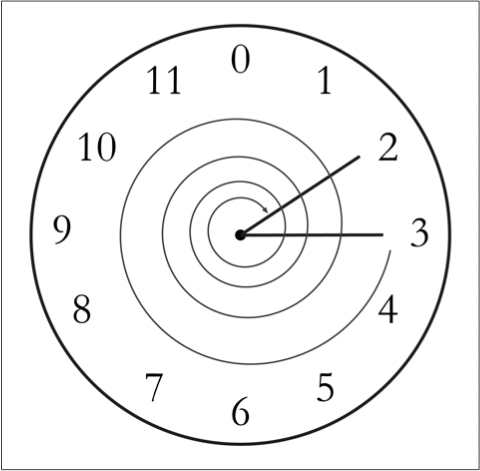
\includegraphics[scale = 0.25,width =9cm]{images/clock.png}
\textbf{To answer the question on previous page we use the modulo operator 
currently it is 3 and we are asked time 47 hours from now. For carrying out this we first add add 47 to 3 (47+3) and then take modulo by 12 since any the value of "hour" has to lie between [0,11] strictly \\
the above  answer  is calculated by (3+47)\%\ 12 = 2 . }

\textbf {Any operation between two variables could be re-written in terms of modulo.}
\\
\
\textbf{Given a modulo number "m" ( in our wrapped clock case m was 12) the operations addition, subtraction,multiplication and division could be re-written this way}
\\
\\
\textbf{ a + b  becomes equivalent to (a+b)\%\ m in case of modulo addition}
\\
\\
\textbf { a - b becomes equivalent to (a-b)\%\ m in case of modulo subtraction }
\\
\\
\textbf { a * b becomes equivalent to (a*b)\%\ m in case of modulo multiplication}
\\
\\
\textbf { a / b becomes equivalent to (a/b)\%\ m in case of modulo division }

\pagebreak 
\section * {FINITE FIELD SETS}
\hrule
\bigskip
\textbf{ We learnt about sets in the first section followed by five  properties of set elements under application of operators like '+','-','*' and '/' .Now we look at finite fields which are a type of set that strictly follow the five properties (closed property,additive identity,multiplicative identity,additive inverse,multiplicative inverse under modulo arithmetic  )}.
\\
\\
\textbf{ In case of a finite field if the size of set is p, all the objects,elements inside the set are strictly from 0 to p-1.\\ \\ Mathematically the finite field set looks like this \\ \\
F(p) = \{0,1,2,3....p-1\} (Read as "a finite field of order  p")
\\ \\
F(p) is called the "Finite field of p" (why finite? because the set has finite elements starting from 0 to p-1 (one less than p)
\\\\ 
F(29) = "Finite field of 29"
F(17) = "Finite field of 17"
the "p" in F(p) is always a prime number 
\\ \\
A finite field of order 11 looks like this \\
F(11) = \{0,1,2,3,4,5,6,7,8,9,10\} \\
A Finite field of order 13 looks like this \\
F(13) = \{0,1,2,3,4,5,6,7,8,9,10,11,12\}
\\
\\
For understanding elliptic curve cryptography which is at the heart of bitcoin transaction we consider and understand finite fields whose order is prime.
}
\pagebreak 
\section * {APPLYING MODULO ARITHMETIC TO FINITE FIELD ELEMENTS}
\hrule
\bigskip 
\textbf{Now we apply the two concepts we read earlier i.e., finite field sets and modulo arithmetic to prove that each element in our finite field satisfies the five property of sets we've discussed earlier ( closure property ,additive identity,multiplicative identity,multiplicative inverse,additive inverse)
\\
Let us consider finite field of 11 i.e., F(11) = \{0,1,2,3,4,5,6,7,8,9,10\} and apply modulo arithmetic to prove five properties 
\\ 
\\
Take any two number from F(11) and add it say take a = 10 and b = 9. We take the modulo with the prime number "p" or the field order 
\\
\\
on addition (10+9) \%\ 11 = (19) \%\ 11 = 9 (which is inside the field)
\\
\\
on subtraction (10-9) \%\ 11 = (1) \%\ 11 = 1  (which also lies inside the field)
\\
\\
on multiplication (10*9) \%\ 11 = (90) \%\ 11 = 2 (which also lies inside the field)
\\
\\
\textbf{Note:}\textit{We will discuss division on finite fields  while proving the multiplicative inverse property for finite fields} 
\\
\\
On taking any two elements from the field and applying first three three binary operators ('+','-','*') with modulo arithmetic for evaluation we see that our closure property satisfies ( which is take any two members from set apply binary operations (we've seen '+','-', and '*') with modulo arithmetic  and the result we get is strictly inside the field.}

\pagebreak 
\section * {APPLYING MODULO ARITHMETIC TO FINITE FIELD ELEMENTS }
\hrule 
\bigskip 
\textbf{The second and third property of  additive identity and multiplicative identity holds by default as we always have 0 and 1 as our elements in our field no matter what set we consider F( of any p) always has 0 and 1 in it  and ‘a’+0 = ‘a’ and ‘a’*1 =’a’ these two cases are always satisfied}
\\
\\
\textbf{ Let's check for the additive inverse property i.e., on choosing any 'a' from the finite field element we get 'a'+(-'a') = 0 
Let's verify it on F(11) = \{0,1,2,3,4,5,6,7,8,9,10\} 
\\
1+(-1) \%\ 11 = 0 \\
2+(-2) \%\ 11 = 0 \\
3+(-3) \%\ 11 = 0 and so on for all members }
\\
\textbf{The final property i.e., multiplicative inverse property is one of the most counter intuitive property we prove. At a first glance it is very non obvious if we go by the definition i.e. we multiply a number from the field with its inverse to get 1 . Let's take 2 as our number now we need to find such a number which exists in the field and on multiplication gives us 1.The only number we could think is (1/2) as 2*(1/2) = 1 . But we see 1/2 is not present in the field itself. So how do we get the intuition? .The answer to the question is given by Fermat's little theorem. Let's look at the theorem.}
\pagebreak 
\section * {FERMAT'S LITTLE THEOREM}
\hrule 
\bigskip
\textbf{Let's us consider  a finite field of any prime order say  F(11) = \{0,1,2,3,4,5,6,7,8,9,10\} \\
Then we  multiply each number in the given set by a number say 'n' (n is strictly greater than  0). Take  n=1, n=2 and n=3 (multiplication here refers to modulo multiplication (n*2) will be (n*2)\%\ p) 
\\ In the first case when we multiply each element by 1 (we exclude 0 since our n should be greater than 0 so our set starts from 1) the resultant set looks something like this \\
\{1 \%\ 11, 2 \%\ 11, 3 \%\ 11, 4\%\ 11, ...... 10 \%\ 11 \}
\\
In the second case when we multiply each element by 2 the resultant set looks something like this \\ 
\{(2*1) \%\ 11 , (2*2) \%\ 11, (2*3) \%\ 11, (2*4) \%\ 11, .... (2*10) \%\ 11 \} 
\\
In the third case when we multiply each element by 3 the resultant set looks something like this \\ 
\{ (3*1) \%\ 11, (3*2) \%\ 11, (3*3) \%\ 11, (3*4) \%\ 11, ....(3*10) \%\ 11 \} 
\\
On evaluating each set the results we get can be seen \\
For n = 1 our final set looks like this \{ 1,2,3,4,5,6,7,8,9,10\} \\ 
For n = 2 our final set looks like this \{
2,4,6,8,10,1,3,5,7,9\} \\
For n = 3 our final set looks like this \{
3,6,9,1,4,7,10,2,5,8\} \\
\\
On carefully examining each set we get we can see that each set just contains all the original elements we started with ( if we write the sets we obtained by multiplying by n=2 and n=3 in ascending order we still get the original set i.e. \{1,2,3,4,5,6,7,8,9,10\} 
\\
\\
From here we can conclude that on modulo multiplication of our field elements by any 'n' which is greater than 0 we get the original field element. This statement can be mathematically written as \\ \\
\{1 \%\ p, 2 \%\ p, 3 \%\ p, 4\%\,p ......(p-1) \%\ p \} = \{(n*1) \%\ p, (n*2) \%\ p, (n*3) \%\ p ......(n* p-1) \%\ p \} for any n which is greater than 0 
\\
}
\pagebreak
\section * {FERMAT'S LITTLE THEOREM}
\hrule 
\bigskip 
\{1 \%\ p, 2 \%\ p, 3 \%\ p, 4\%\,p ......(p-1) \%\ p \} = \{(n*1) \%\ p, (n*2) \%\ p, (n*3) \%\ p ......(n* p-1) \%\ p \}
\\
\\
\textbf{Since  same numbers are in
both sets. We can then multiply every element in both sets to get this equality
\\
\\
(1*2*3*4*5*6*7...p-1) \%\ p = (n*2n*3n*4n*..(p-1)*n) \%\ p
\\
\\
On the left side the term (1*2*3*4*5....p-1) can be written as factorial of p-1 \\
On the right side  (1*2*3*4*5....p-1) again  can be written as factorial of p-1 and since we have  multiplied the term 'n'  p-1 times on the right side  (n*n*n.. p-1 times) that term becomes n raised to power p-1 \\ \\ 
our equation now becomes:} 
\\ 
\\ 
\textbf{\[ (p-1)! \%\ p = ((p-1)! * n^{p-1}) \%\ p   \] }
\textbf {The (p-1)! terms on left hand side and right hand side gets cancelled out and our final expression becomes as :}
\\
\\
\textbf{\[ 1 \%\ p = (n ^{p-1}) \%\ p \]}
\\
\\
\textbf{Which is the Fermat's little theorem}

\pagebreak
\textbf{We've proved the Fermat's little theorem on the previous page but the entire idea  of doing so is to see how multiplicative inverses are calculated inside the field 
\\
Another important bit of information that we have to keep in mind is that we've not yet proved the closure criteria for division (modulo division) of two finite field elements.Proving closure under division using Fermat's theorem will give us the perfect premise for understanding multiplicative inverse. So let's use the Fermat's theorem to prove closure property of finite fields under division (i.e., take any two 'a' and 'b' from field and perform (a/b) \%\ p the result still lies inside the field)}
\\
\textbf{Let's consider our old friend field F(11) = \{0,1,2,3,4,5,6,7,8,9,10\} and take any two numbers say 'a' = 5 and 'b' = 6 and perform modular division (5/6) \%\ 11. Intuitively we see that there is no way that the result lies on the field itself. One thing to note here is that the operation (a/b) can also be written as a * b inverse (power of b on the denominator is 1 when it comes to numerator the power becomes -1)}
\textbf{\[((a^{1}/b^{1})\%\ p) = (a^{1}* b ^{-1}) \%\ p \]}
\textbf{We know what the value of 'a'   but we don't know what the value of b inverse  is so here we use the Fermat's Theorem to find it. Rewriting the Fermat's theorem  }
\\
\textbf{\[ 1 \%\ p = (n ^{p-1}) \%\ p \]}
\textbf{ In the above term 1 \%\ p can be simply written as 1 }
\textbf{\[ 1  = (n ^{p-1}) \%\ p \]}
\textbf{Also b inverse can be written as b inverse * 1 (any number can be written as number * 1)}
\textbf{\[ (b^{-1}) =  (b^{-1} *1)  \]}
\\
\textbf{we can replace the value of 1 in the above equation by the value of 1 we have obtained in Fermat's little theorem. On doing so  }
\textbf{ \[ b^{-1} =(b^{-1} *  n ^{p-1})  \%\ p \] }
\textbf{Now since we know n is any number greater than 0 n could be b  as well or n could be a or  n could be replaced by any number greater than 0.On replacing n by b we get }
\pagebreak
\textbf {\[ (b^{-1}) = (b^{-1} * b^{p-1}) \%\ p \]  }
\textbf{we know when two bases are same power can be added ( a power p * a power p can be written a  power (p+p) similarly  here on the right hand side of the above equation  b power -1 and b power p-1 can be written as b power -1+p-1 so rewriting the equation we have }
\textbf {\[ (b^{-1}) = (b ^{-1 + (p-1) = p-2}) \%\ p \]}
\textbf {Finally the result we get for b inverse is }
\textbf {\[ (b^{-1}) = (b ^{p-2})\%\ p \] }
\textbf {Above we have the value of b inverse that we have obtained using Fermat's little theorem now we come back to our original problem which we started with that is modulo division of finite field. We had taken our a as 5 and b as 6, the field under consideration was F(11) p = 11. (a/b) \%\ p could be written as (a * b inverse) \%\ 11 . Now that we know how to find the value of b inverse let's find it using the above equation}
\textbf {\[ 6 ^{-1}  = 6 ^{11 -2} \%\ p \]}
\textbf{\[6 ^{-1} = 6 ^{9} \%\ p \]}
\textbf {\[6 ^{-1} = 10077696 \%\ 11 \]}
\textbf {\[6 ^{-1} = 2\]} 
\textbf {\[ (5/6) \%\ 11 = (5 * 6 ^{-1} ) \%\ 11 \]}
\textbf {\[ (5/6) \%\ 11 = (5 * 2 ) \%\ 11 \]}
\textbf {\[ (5/6) \%\ 11 = 10 \]}
\textbf { We see that the result we obtained above (10) lies inside the field. This might not be super-intuitive at the first place but on circling back to the derivations and proofs the ideas start to make sense. Also the whole idea of doing this was to find out the multiplicative inverse which magically we've already done i.e., the value of b inverse we've found out in the above equation is the way the multiplicative inverse of any number from the field. We shall now be showing a few examples how we take  a number and multiplying it with the multiplicative inverse gives us 1 ( this was the criteria for multiplicative identity) }

\pagebreak 
\section * {EXAMPLES}
\textbf {Given a finite field F(11) = \{1,2,3,4,5,6,7,8,9,10\} prove multiplicative identity for 4 also show  (7/8) lies inside the field}
\\
\textbf {Let's prove multiplicative identity first}
\textbf {Let b = 4. We find b inverse first We know that :}
\textbf{\[b ^{-1} = (b ^{p-2})\%\ p \]}
\textbf{\[4 ^{-1} = (4 ^{9}) \%\ 11 \]}
\textbf{\[4^{-1} = 262144 \%\ 11 \]}
\textbf{ \[4^{-1} = 3 \]}
\textbf{ Now that we've found out that inverse of 4 is 3 to prove the multiplicative identity we must show that (a * a inverse) \%\ p  should strictly be 1 and 'a' shouldn't be 0 as multiplicative inverse of 0 does not exist}
\textbf{(4 * 3 ) \%\ 11 = (12) \%\ 11 = 1  which proves the multiplicative identity.Similarly we can prove it for 5 and 6 as well and any number in the field}
\textbf{ Now we see that modulo division follows closed property ( i.e., (a/b) \%\ p lies inside the field itself. Let's take the example of (7/8) }

\textbf {\[(7/8) = (7 * 8^{-1})\]}
\textbf { Since we know that }
\textbf {\[b^{-1} = b ^{p-2} \%\ p \]}
\textbf {\[8 ^{-1} = 8 ^{11-2} \%\ 11 \]}
\textbf {\[8 ^{-1} = 134217728 \%\ 11 \]}
\textbf {\[8 ^{-1} = 7 \]}
\textbf {\[(7* 7) \%\ 11 = 5\]}
\textbf { we see that on division we get 5 which strictly lies inside the field you can now take other examples and verify for yourself.Now that we have verified closure( modulo addition, subtraction, multiplication, division of any two finite field elements always lies inside field),additive identity (a + 0 = 0 ), multiplicative identity (a* 1 = a), additive inverse (a +(-a) = 0) and multiplicative inverse ( a* a inverse =1),we are now ready to look forward to a new topic. }

\pagebreak





\end{document}






